\chapter{Reinforcement-Learned Balancing}
\label{chap:ns}

\section{Introduction}
A significant goal of the yearly progression of RoboCup robotics is the improvement of bipedal locomotion and stabilisation. Such bipeds are expected to execute many different movement behaviours and switch between them seamlessly without falling over -- the type of responsiveness expected in playing a game of soccer. 

We explore an approach to robot self-stabilisation using multi-goal Reinforcement Learning. This approach is applied to learn the side-to-side (lateral) movement of a bipedal robot in simulation. Applied to the Naos, this allows for self-stabilisation without the need for difficult hard-coded solutions in a variety of different behaviours, including: changing support feet at different frequencies; standing upright; standing on either foot; and switching between these behaviours. These behaviours are then stable and able to respond optimally to dynamic disturbances and when switching.

\section{Background \& Literature Review}

\section{Theory \& Methodology}

Team rUNSWift's 2013 Robocup Open Challenge entry was titled \textit{``Stability Control through Machine Learned Behaviours''}\cite{openchallenge}.

We begin by defining a robot model, including as much accuracy in the links, joints, masses, etc. as possible -- an example of this is seen in Figure \ref{fig:lean}. We define the robot stabilisation state and establish cost functions in the form of goal behaviours (such as standing upright, for example), and state transitions as random action exploration, able to automatically identify the system model (i.e. we do not assume an inverted pendulum model). 

The reinforcement learning then learns the actions required for optimal stabilisation of given behaviours, as well as for the transition between behaviours. These actions are used in the creation of policies, which define the action required for each possible state of the robot. Some simplified example policies can be seen in Figure \ref{fig:policy}.

The policy tables are then interpreted by the real-world Nao robots, allowing them to mimic the behaviour seen in the simulation by actuating joints to follow the optimal action sequence.

\section{Results}
For the RoboCup 2013 Open Challenge we plan to demonstrate a robot which is able to self-stabilise with various behaviours, including standing on one leg and jogging on the spot. The robot is also able to seamlessly and optimally transfer between these behaviours while maintaining a stable body, something already exceedingly difficult in manual hand-coding of behaviours.

Most importantly, we plan to show the continued stability of a robot even when reacting to disturbances, such as being bumped by another robot. Given the dynamic behaviour of such disturbances, hand-coding is virtually impossible or relies on extensive trial-and-error manual tuning -- whereas this is simply a property of the learned optimal policies for any behaviour, therefore guaranteeing simple automatic stabilisation of the robots after policy learning.

\begin{figure}[!t]
\centering
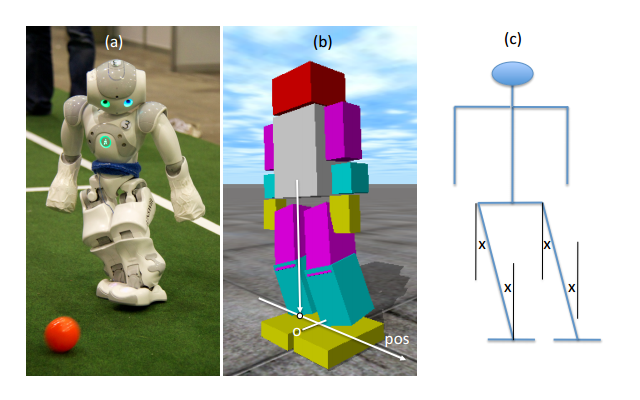
\includegraphics[width=3.5in]{img/RL_lean.png}
\caption{We model the Nao robots in (b) as a $23 DOF$ (Degree Of Freedome) system. \cite{bernhard_rl}}
\label{fig:lean}
\end{figure}


\begin{figure}[!t]
\centering
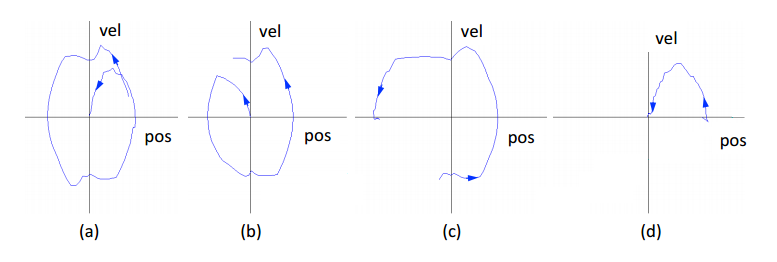
\includegraphics[width=3.5in]{img/RL_policies.png}
\caption{Simplified example of learned policies. Here we see the transition functions between the behaviours of: (a) switching between a slow walk-on-the-spot to standing upright; (b) standing upright to walk-on-the-spot; (c) walk-on-the-spot to standing on right leg; (d) standing on left leg to standing upright.}
\label{fig:policy}
\end{figure}


\section{Evaluation}
\section{Future Work}
\section{Conclusions}
